\chapter{Predicting susceptibility to tuberculosis based on gene expression profiling}\label{ch:comp}

\section[Abstract]{Abstract\footnotemark}


\footnotetext{Citation for chapter: Manuscript in Prep}

\section{Introduction}\label{ch03-introduction}

\section{Results}


\section{Discussion}


\section{Methods}



\clearpage


\subsection{Supplementary Figures}\label{ch03-supplementary-figures}

\begin{figure}[!htb]
\centering
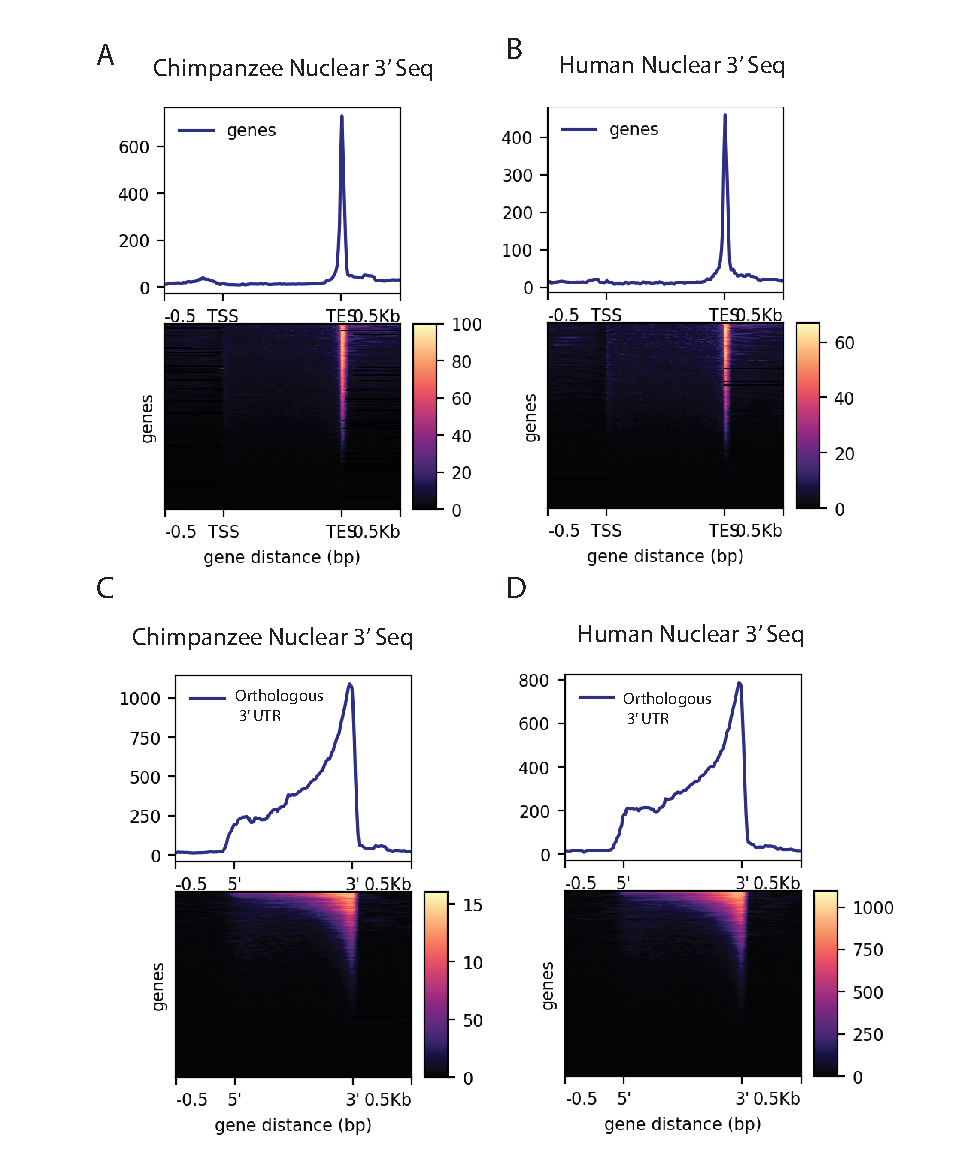
\includegraphics[width=5in]{img/ch03/Fig1-figSup1.pdf}
\caption[Density of merged human and chimpanzee 3' Seq]{\textbf{Density of merged human and chimpanzee 3' Seq} \bf{(A)}  Coverage of 6 chimpanzee, nuclear 3' seq reads along Refseq transcripts {\bf (B)} Coverage of 5 human, nuclear 3'seq reads along Refseq transcripts \bf{(C)} Coverage of 6 chimpanzee, nuclear 3' seq reads orthologous 3' UTRs \bf{(D)} Coverage of 5 human, nuclear 3' seq reads orthologous 3? UTRs}
\label{fig:ch03-deeptools}
\end{figure}
\clearpage

\begin{figure}[!htb]
\centering
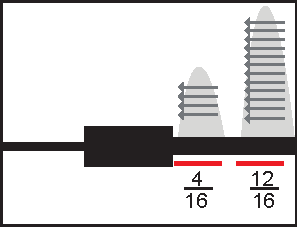
\includegraphics[width=5in]{img/ch03/Fig1-figSup2.pdf}
\caption[Model representation of usage calculation]{\textbf{Model representation of usage calculation}Representation of PAS usage calculation. Usage is a ratio of reads at each PAS to the number of reads mapping to any PAS in the same gene. Adapted from \ref{ch:QTL}}
\label{fig:ch03-UsageCalc}
\end{figure}
\clearpage

\begin{figure}[!htb]
\centering
\includegraphics[width=5in]{img/ch03/Fig1-figSup3.pdf}
\caption[PAS usage is highly correlated across species]{\textbf{PAS usage is highly correlated across species} \bf{(A)} Correlation between human and chimpanzee PAS usage for 44,432 PAS. Red line is a 1:1 line. Linear regression line and Pearson?s correlation plotted in blue. \bf{(B)} Pairwise correlation for human and chimpanzee PAS usage.}
\label{fig:ch03-UsageCorr}
\end{figure}
\clearpage

\begin{figure}[!htb]
\centering
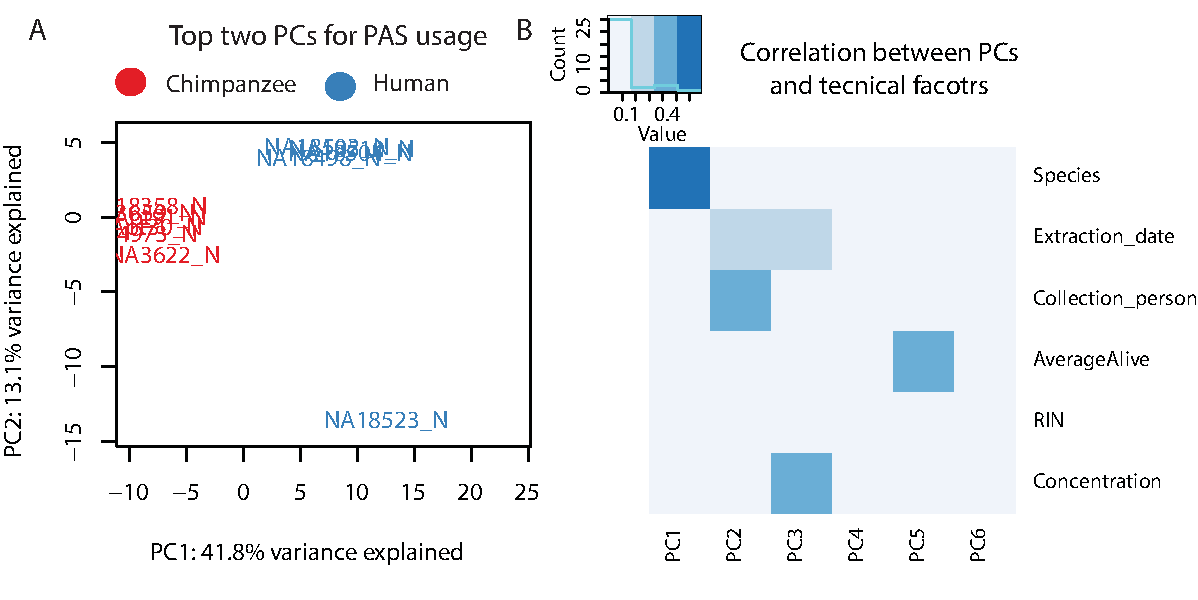
\includegraphics[width=5in]{img/ch03/Fig1-figSup4.pdf}
\caption[Variation in PAS usage]{\textbf{Variation in PAS usage}\bf{(A)} Plot of first two principal components \emph{(PCs)} calculated by a principal component analysis on PAS usage (44,432 PAS). Chimpanzee samples are shown in red and human samples are shown in blue \bf{(B)} Heatmap representing correlation between technical factors and PCs. Y axis factors include: Species, Extraction date, Collection person, AverageAlive (average of two live dead calculations at time of collection), RIN score, RNA concentration. Explanation of factors and values in supplemental table \ref{tab:ch03-s1}}
\label{fig:ch03-PCAthreeprime}
\end{figure}
\clearpage

\begin{figure}[!htb]
\centering
\includegraphics[width=5in]{img/ch03/Fig1-figSup6.pdf}
\caption[Number of PAS per gene largely conserved between species]{\textbf{Number of PAS per gene largely conserved between species} Histogram of the number of PAS detected at 5\% usage in human minus the number of 5\% usage in chimpanzees. Red vertical line represents mean difference (0.39).}
\label{fig:ch03-SpecPASnum}
\end{figure}
\clearpage


\begin{figure}[!htb]
\centering
\includegraphics[width=5in]{img/ch03/Fig1-figSup7.pdf}
\caption[Figure 1B separated by genic location]{\textbf{Figure 1B separated by genic location} Mean PhyloP scores for PAS regions (yellow) and 200 base pair bins upstream and downstream of PAS (orange). A one-sided Wilcoxon test was used to test for increased PhyloP in PAS regions  (Coding region (cds): $p < 2.2x10^{-16}$, 5 kb downstream of genes (end): $p = 7.02x10^{-6}$, intron: $p=0.99$, 3' UTR (utr3): $p < 2.2x10^{-16}$, 5' UTR (utr5): $p = 0.011$).}
\label{fig:ch03-phylopLoc}
\end{figure}
\clearpage

\begin{figure}[!htb]
\centering
\includegraphics[width=5in]{img/ch03/Fig1-figSup8.pdf}
\caption[PAS with AATAAA and ATTAAA are used more often]{\textbf{PAS with AATAAA and ATTAAA are used more often} Mean PAS usage of the top two signal site motifs in human and chimpanzee plotted by annotated signal site.}
\label{fig:ch03-SignalUsage}
\end{figure}
\clearpage

\begin{figure}[!htb]
\centering
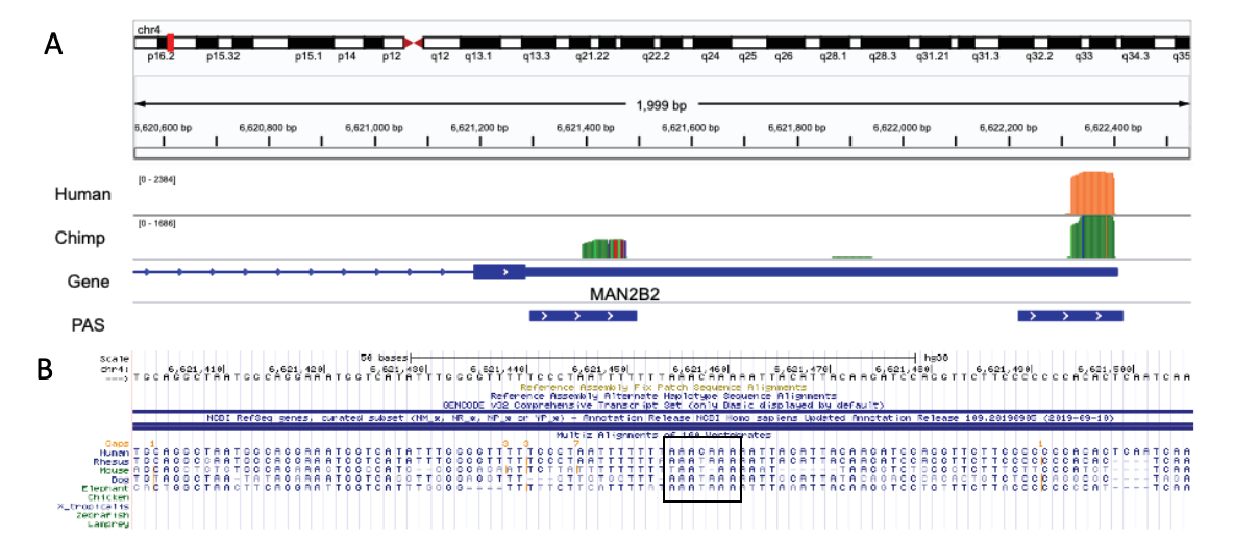
\includegraphics[width=5in]{img/ch03/Fig1_figSup9.pdf}
\caption[Chimp specific PAS likely due to loss of signal site in human lineage]{\textbf{Chimp specific PAS likely due to loss of signal site in human lineage} \bf{(A)} IGV track for example of a chimpanzee specific PAS in MAN2B2 gene. Top track is merged coverage from 5 human nuclear 3' seq libraries. Chimp track is merged coverage from 6 chimpanzee nuclear 3' seq libraries lifted to human genome with CrossMap \citep{ } \bf{(B)} Sequence alignment for region upstream of proximal PAS from UCSC genome browser \citep{kent_human_2002}.Black box indicates the signal site location. Canonical signal site is the ancestral state and was lost in the human lineage.}
\label{fig:ch03-exChimpspec}
\end{figure}
\clearpage


\clearpage
\section{Supplementary Tables}\label{ch03-supplementary-tables}

\begin{table}[!htb]
\caption[3' Seq metadata]{\textbf{3' Seq metadata} 
(see supplementary file associated with this dissertation) Metadata for 3' Seq data. Column names as described- Species:Cell line species , Lines: Cell line ID, Fraction: Cellular fraction, CollectionDate: Date of cell harvest and nuclear isolation, Extraction\_date: Date of RNA extraction, Collection\_person: Author initial for who processed cell harvest and nuclear isolation, UndilutedAverage: Average of 2 cell count measurements $1x10^6$, AverageAlive: Average of 2 cell live dead counts - calculated with trypan blue stain, Concentration: Extracted RNA concentration (ng/ml), RIN: RIN score for extracted RNA, 260.280.Ratio: 260/280 ratio calculated on nanodrop, Library: 3' Seq library date, Reads: Number of sequenced reads, Mapped\_wMP: Number of Mapped reads before removing reads likely due to misprimming, Mapped\_Clean: Number of Mapped reads after removing reads likely due to misprimming}
\label{tab:ch03-s1}
\end{table}


\begin{table}[!htb]
\caption[Expression Independent eQTLs]{\textbf{RNA sequencing metadata} 
(see supplementary file associated with this dissertation) Metadata for RNA sequencing data. Column names as described- Species:Cell line species , Lines: Cell line ID, Collection\_person: Author initial for who processed cell harvest and nuclear isolation, UndilutedAverage: Average of 2 cell count measurements $1x10^6$, AverageAlive: Average of 2 cell live dead counts - calculated with trypan blue stain, CollectionDate: Date of cell harvest and nuclear isolation, Extraction: Date of RNA extraction,  RIN: RIN score for extracted RNA, BioAConc: RNA concentration (ng/ul), Reads: Number of Sequenced reads, Mapped: Number of mapped reads, AssignedOrtho: Number of mapped reads assigned to orthologous exons.}
\label{tab:ch03-s2}
\end{table}

